\section{Research}

\subsection{Music Technology}

\subsubsection{MIDI}

MIDI stands for Musical Instrument Digital Interface, and it is used to communicate music
to computers in separate parts. MIDI files themselves do not contain any audio. Instead,
they send system and channel messages. Each message describes several features, but in
this project we are primarily concerned with note ON/OFF and the timing clock. The note
ON/OFF tells which notes are playing during a certain event and at what velocity. The
timing clock keeps track of when each event is scheduled to occur.

Between these two features we can determine pitch, timing, and expression - the three
components of a note which determine whether or not it is melodic in context.

\subsubsection{DAW}
\label{sec:daw}

DAW stands for Digital Audio Workstation. DAWs are the software that provide an interface
through which users can alter the contents of a MIDI or other audio file. Because our DAW
is to be isolated to a MIDI controller, it  will only contain functions concerning MIDI
data. When dealing with MIDIs, DAWs visualize audio in a piano roll display. The
foundation of the piano roll is a set of rows, each one representing a piano key and its
corresponding note. The horizontal axis represents the timing clock data. For each note
that plays in the MIDI, the piano roll displays a colored bar located in the row of the
corresponding note and spanning the length of the corresponding timing clock data.
Additionally, some DAWs show the velocity of the note by the color of the bar - most
commonly, red denotes high velocity while blue/violet denotes low velocity.

\begin{figure}[h!]
  \centering
  \includegraphics{image/PianoRoll.png}
  \caption{Example of a piano roll display}
  \label{fig:piano_roll}
\end{figure}

The most basic ways a DAW can alter a MIDI are by adding, deleting, and editing notes on
the piano roll; users can change the timing, pitch, and/or velocity of any note. DAWs can
also quantize notes, meaning they will automatically shift the timing of the notes so that
every note begins on some specified fraction of the tempo (most commonly a thirty-second
note). This function is especially useful in adjusting for human errors in timing when
writing MIDIs with a MIDI controller. Better timing makes it easier to synchronize with
other tracks that might end up in the same audio file.

\subsection{Music Theory: Consonance}

One of the biggest issues with creating computer-generated music is that music, like all art
forms, is highly subjective. There are no universal rules for right or wrong, and yet at the
same time there are combinations of sound that could (almost) universally be considered bad music.
So how does a computer decide what factors will most likely lead to a good melody?

To start, the generally agreed upon definition of melody is that it is the linear succession
of musical tones, with its primary components being pitch and rhythm. Occasionally, it also
encompasses tonal color and other factors of expression.\autocite{melody} In music theory, parts
of music can be described as dissonant or consonant. Dissonance denotes a feeling of instability or
incompleteness in a musical phrase, and consonance denotes resolution and stability. Once again,
these metrics are highly subjective, but they are based in the principle that music is composed
of organized patterns in sound.\autocite{musiciansArithmetic} Aside from easily identifiable
patterns, such as rhythm or repeated note sequences, this especially applies to patterns in note
intervals.

\subsubsection{Scales}

The standard tuning for fixed-pitch instruments - piano keyboards included - is called twelve-tone
equal temperment tuning (often shortened to 12TET). A primary basic pre-requisite to notes being
considered tonally consonant is whether or not they come from the same key as their context.

\subsubsection{Harmonics}

Scales are not the only markers for tonal intervals. Another factor that plays a role in the
consonance of pitch is harmoncics. The Lipps-Meyer law, for example, proposes that the consonance
of a melodic interval can generally be determined by whether or not the end tone of the interval
can be represented by a power of two.\autocite{musiciansArithmetic} These numbers which represent
the tones are not their scale intervals, but instead are derived from the Harmonic Series.

The Harmonic Series is actually based on a principle in physics. Sound is a wave, any tone \textit{t}
is a sound wave oscillating at a specific frequency \textit{f}. Any sound wave with a frequency
that is an integer multiple of \textit{f} is considered to be harmonic to \textit{t}.\autocite{intervals} For example,
if \textit{f} is the frequency of the tonic (the root note of a scale), the unison (no interval,
so also the root note) would be the first harmonic because it has the same frequency. The second
harmonic has a frequency of 2\textit{f} - this coincides with the tone that's exactly one octave
above the root. In fact, every power of two falls on the root note of a different octave. Going
back to the Lipps-Meyers law, this implies that proper consonance can be achieved by ending the
musical phrase on the tonic of the key.

\begin{figure}[h!]
  \centering
  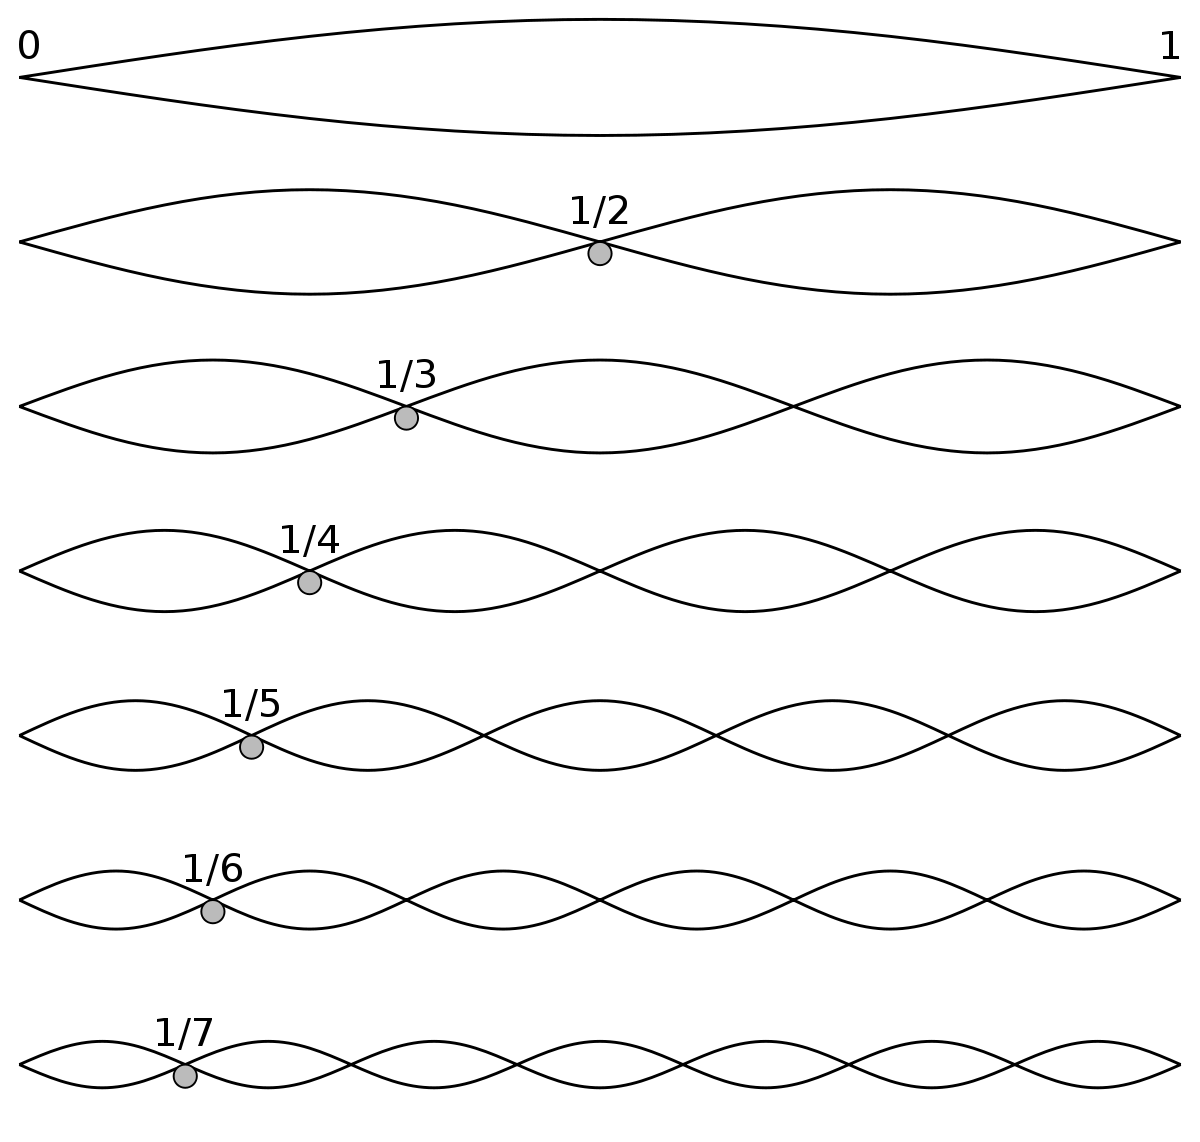
\includegraphics[width=0.5\linewidth]{image/Harmonics.png}
  \caption{A comparison of the wavelengths of waves in a Harmonic Series \autocite{harmonicSeries}}
\end{figure}

\begin{table}[h!]
  \centering
  \resizebox{0.5\textwidth}{!}{%
  \begin{tabular}{|l|l|l|l|l|l|}
  \hline
  \multicolumn{5}{|l|}{\textbf{Harmonic}} & \textbf{12TET Interval}        \\ \hline
  1     & 2     & 4     & 8      & 16     & prime (octave)                 \\ \hline
        &       &       &        & 17     & minor second                   \\ \hline
        &       &       & 9      & 18     & major second                   \\ \hline
        &       &       &        & 19     & minor third                    \\ \hline
        &       & 5     & 10     & 20     & major third                    \\ \hline
        &       &       &        & 21     & fourth                         \\ \hline
        &       &       & 11     & 22     & \multirow{2}{*}{tritone}       \\ \cline{1-5}
        &       &       &        & 23     &                                \\ \hline
        & 3     & 6     & 12     & 24     & fifth                          \\ \hline
        &       &       &        & 25     & \multirow{2}{*}{minor sixth}   \\ \cline{1-5}
        &       &       & 13     & 26     &                                \\ \hline
        &       &       &        & 27     & major sixth                    \\ \hline
        &       & 7     & 14     & 28     & \multirow{2}{*}{minor seventh} \\ \cline{1-5}
        &       &       &        & 29     &                                \\ \hline
        &       &       & 15     & 30     & \multirow{2}{*}{major seventh} \\ \cline{1-5}
        &       &       &        & 31     &                                \\ \hline
  \end{tabular}}
  \caption{The relationship between Harmonic and 12TET intervals}
  \label{Tab:harmonic_intervals}
\end{table}

Basically, in a roundabout way, we've affirmed a fairly core and commonly known principle of
melody writing: resolve to the root. However, this is not the only way in which interval patterns
and the Harmonic series are used to determine consonance. Octaves are not actually the only case to
which the Lipps-Meyers law applies. Melodic intervals can be simplified the same was fractions can.\autocite{intervals}
So then, an interval of 9:6, which correlate to the major second and major fifth respectively, could
also be written as 3:2 and therefore follows the Lipps-Meyers law.

Another theory on the relationship between harmonics and dissonance was proposed by physicist
Herman von Helmholtz, who posited that the "beats" created by the resonance of two tones which are
close in frequency can help us quantify the dissonance of an interval.\autocite{intervals} Though it is now regarded
that Helmholtz's theory incompletely addresses the nuances of modern physics and music, it is
a valuable discussion because it provides a foundation from a simplified understanding. Because
of its simplicity, we can more clearly view the connections between harmonics and dissonance and
more easily frame it in a way we might be able to apply with computers which also lack such nuance.
An important part of Helmholtz's theory was that harmonic intervals of smaller integers tend to
create higher degrees of consonance.\autocite{intervals} This much is evident in common chord
structures. For example the major tonic is composed of harmonics 1, 3, and 5. Conversely, the
diminished tonic - commonly viewed as more dissonant - is composed of the harmonics 1, 11, and 19.

\subsection{AI}

Our original concept for the AI model took a computer vision approach. To begin we would
have had to develop a script which could convert between MIDI data and a PNG
visualization. This image would be similar in structure to what might show on the piano
roll display of a DAW. Each pixel along the vertical axis would represent a key on the
MIDI controller, and each pixel along the horizontal axis would represent some small
fraction of a beat - hypothetically the length of a sixty-forth note, as this is the
shortest common time interval in music. The hue of each pixel would denote the velocity
of the note being played at that time and pitch - a black pixel would mean no note is
being played while a white pixel would show a note being played at maximum velocity.
These images could then be fed into a Convolutional Neural Network (CNN) which would
replicate the visual patterns and thereby output an image that can be converted back into
a MIDI of a completed melody.

\begin{figure}[h!]
  \centering
  \includegraphics{image/MIDIsample.png}
  \caption{Example of a visualized MIDI file}
  \label{fig:midi_sample}
\end{figure}

This approach was originally considered for its advantages over a more direct MIDI-based
AI. For starters, when conducting some test trials, it was found that the PNG
visualizations are about a quarter the file size of the original MIDIs they were converted
from. This, in conjunction with the comparatively easy calculations of a CNN on a
simplistic bitmap, suggested that a computer vision model would be fast to train.

Additionally, patterns in music are much easier to recognize through visualization than
through note data. Much of the music theory that determines whether a note is melodic in
context is generalized in that it works according to intervals as opposed to discrete
relationships between specific notes. MIDI files don't provide any information about
scales or chords; they simply list which notes were played. It might take an AI a good bit
of to recognize that the interval between C and E is the same as the interval between F
and A - and even longer still to determine which intervals are musically dissonant or not,
and in which contexts. When music is visualized, however, it can generalize the same way
it does in abstract theory. Melodic intervals appear visually the same, regardless of the
root note. So rather than having to learn separately that C pairs well with E and F pairs
well with A, it can generalize that any note will pair well with the note that is four
semitones (or in the AI's case, four pixels) above it, known in music theory as the major
third.

The computer vision model was also favored for its level of technical skill. As students,
we have been exposed to the concept of CNNs but have not yet had the opportunity to apply
them. This model felt appropriate for our skill level because it is centered around a
technique we already understand, but it also implements that technique to a degree we have
never attempted before.

\subsubsection{PixelCNN}

For the computer vision model, our lead candidate was PixelCNN. Like a standard CNN,
PixelCNN processes its image inputs primarily through layers of masked convolution.
The "masks" used in the convolution layer are square matrices, and each element of the matrix
is a numerical value that denotes the weight of that element. These masks are iterated over the
input image, convolving with the brightness of the pixels under the mask. In colored images,
the process is repeated once for each color channel: red, green, and blue.\autocite{pixelCNN} Depending on the
configuration of the weights in the matrix, different masks can be used to identify different
visual patterns. Each convolution with each mask outputs a two-dimensional array of values
called a feature map.

Unlike a standard CNN, however, PixelCNN specifically uses masks that only allows it to read
one pixel at a time: row by row, and left to right in each row.\autocite{pixelCNN} This enforces that each pixel
is dependent upon only those above and to the left of itself. Using this unique relationship,
PixelCNN has a unique use-case in predicting the bottom half of an image after processing the
top half as input. The AI uses the probability distribution of visual features found in all pixels
iterated through prior to inform the probability distribution it creates to predict the pixels that
will follow.\autocite{pixelRNN}

\begin{figure}[h!]
  \centering
  \includegraphics{image/PixelMask.png}
  \caption{PixelCNN's unique mask prevents the AI from peeking ahead}
  \label{fig:pixel_mask}
\end{figure}

This made PixelCNN a particularly appropriate candidate for our computer vision model
because completing an image after processing the first half is exactly the mechanic we
planned to use to achieve the melody autofill. All we would have to do is rotate the input
image such that the time axis propagates top to bottom as opposed to left to right.
Additionally, the dependencies that PixelCNN establishes simulate dependencies in music
really well. Whether or not a note is melodic depends on its context - specifically, the
notes that came before it in time as well as the other notes being played at the same
time. Adjusting the axes, PixelCNN's dependency upon all pixels above equates to the
current note being dependent on all notes that were played before it. As for its left to
right dependency, chords are typically built upward from the root - which, when rotated,
would be left to right.

Our main challenge in the use of PixelCNN would be the collection and preprocessing of
training data. For this model to work for our purposes, we would have to convert each MIDI
file into a piano roll visualization which is rotated 90 degrees clockwise.

\subsubsection{Magenta}

As an alternative, we could use an existent open source solution. Magenta is an open
source project for artistic applications developed by Google AI\autocite{magentaHome}.
This project has released in 2018 an extensive AI library for art and music. This one,
contains already trained models, API and datasets that can be directly used to solve our
problem. Although, the level of functionalities already included in these libraries can
defeat the academic purpose of the current project, there are valuables tools to create
our own autocomplete AI model. The project offers blank models to be trained by our own
set of data, and also offers the posssibility of using pre-trained models.

As an already functional solution that can be directly applied to our work without any
modification is the module MusicRNN\autocite{musicRNN}. This one contains three models of
interest: MelodyRNN, ImprovRNN, and PerformanceRNN. All these models, as their name
implies, are based on recurrent neural netoworks (RNN) produced with Google's TensorFlow.

In constrast with the already mentioned CNN, that processes grid values as is a picture,
RNN processes sequential data as string of caracthers, words, or in our case of
interest, melody representations. RNN also considers proccesed information along large
sequnces of data, and not purely local extent as CNN.\autocite{fundamentalML}

\paragraph{MelodyRNN.}
MelodyRNN model generates melody based on an input melody. To achieve this, it uses
language modeling (probability distribution over a sequence of data) with long short-term
memory (LMST) networks. This is a variant of RNN design to improve the performance of
regulr RNN across large sequnces of data. The main issues that LMST adress are those
related to the exploding and vanishing gradients magnified on any recursive network due to
the accumulation of errors on the successive feedbacks of data analysis. This models also
have four configurations to assists determining the range of pitches, indentifying
recursive patterns, and pay special attention on specific sections of the input melody.
\autocite{melodyRNN}

This model could be in charge of the autocomplete feature we are
looking to achieve in our project.

\paragraph{ImprovRNN.}
ImprovRNN generate melodies in the same fashion of MelodyRNN. The main difference with the
before model is the conditionment of the generated melody to a chord progression. This
model counts with similar set of configurations than MelodyRNN, but with the addition of
usign as inputs vectors representing chords of the progression. Although, this can be a
interesting feature to generate melodies, the model requires to encode the full input
melody in XML format, not supporting direct MIDI input.\autocite{improvRNN}

This model would not be directly applied to our project, but still could add interesting
features for an expanded instance.

\paragraph{PerformanceRNN.}
PerformanceRNN generates melodies using dynamic and expressing timing. This allows to
generate more natural feeling as if a real player is adding to the expression of the
performance. Although, this came with some trade off as some keys can fall outside the
proper timing. \autocite{performanceRNN}

This model add a nice to have feature, but is not fundamental for our first aproach.

\paragraph{Datasets.}
Magenta project offers a set of collections of data that has been used to pre-train
models. From ths collection, seems that the MAESTRO (MIDI and Audio Edited for Synchronous
TRacks and Organization) dataset could be the most useful for this project. It contains
over 200 hours of key annotated piano performing. Other set that can be useful for our
classical music appoach is the Bach Doodle Set. A large audio dataset (over 6 years of
total audio), collected by Google using its Bach Doodle. \autocite{magentaData}

The selction of the dataset would be conditioned by the available trianing capabilities
for this project.


\subsection{Embedded Controller Comparisons}
\label{sec:embedded_controllers}

\blindtext

\subsection{DAW Frontend Technologies}

We are looking to use a browser-based frontend Design. This approach is ideal for its ease
of implementing a user interface as well as its cross-platform compatibility. Should we
decide to make the software even more portable by isolating it from the MIDI controller,
it will be viewable on any device that can run a browser. And because of the computational
limits of the MIDI controller, any modern device that is suited for a browser will
inherently be able to run the MIDI autofill software as well.

Our first consideration was React. Considering our group's familiarity with JavaScript as
well as HTML and similar markup languages, it would be easier to work with. However, we
ultimately opted to use Flutter. Flutter's default stylization is sleek and fits in well
with the modern aesthetic of technology. Plus, its widgets allow for more polish on a UI
that also has more niche functionality.

As established in \textbf{\ref{sec:daw} \nameref{sec:daw}}, the primary aspect of the UI
will be the piano roll display. The frontend will be responsible for reading the MIDI
messages and converting the note ON/OFF and timing clock features into the position and
dimensions of an arbitrary number of UI elements - each representing a note which can be
edited.

\subsection{Raspberry Pi}

As mentioned in \textbf{\ref{sec:embedded_controllers} \nameref{sec:embedded_controllers}},
the Raspberry Pi is mini-computer which can also function as an embedded controller. The
model we're interested in is the Raspberry Pi 4B, which is the latest model and has the
best hardware. After an analysis of other solutions, we have decided that the
Raspberry Pi is the best fit for our project. To that end, we have researched how the
Raspberry Pi can be configured for use in our project.

\subsubsection{Operating System Choice}

The first configuration choice that needs to be made is the operating system. A Raspberry
Pi out of the box has no operating system. An image must be flashed to an SD card to make
the Raspberry Pi useful. Raspberry Pi's typically run some form of Linux. The Raspberry Pi
4B model uses the AArch64 architecture. It can run most AArch64 based Linux distros, but
we must limit ourselves to armv7 (32 bit) operating systems, as tensorflow does not
natively support AArch64 as of the time of writing. Tensorflow lite supports AArch64, but
tensorflow-lite has a limited number of supported operations, which can inhibit our
development. There are still many OS choices available, as there are many flavors of Linux
that can run on the armv7 architecture. Some common choices for Raspberry Pi include
Raspberry Pi OS (formerly known as Raspian), Arch Linux ARM, and DietPi. Each OS has its
advantages and drawbacks, and it is important for us to select a distro that is well
suited for our use case. We will need to modify the system heavily for our purposes, but
we need a good baseline for modification.

We need our distro to be a lightweight bootloader for our application. There are many
examples of highly specialized distros designed for one specific task. Examples
include RetroPIE, which is used to run retro video games, or OpenMediaVault, which is used
to turn the device into a networked storage device. This is similar to what we want our
operating system to do. Our use case for the Raspberry Pi is to run one specialized
application that we ourselves develop. It should boot straight into our application with
no other UI from the operating system. The best solution for us is to have a custom distro
just for running our application. Developing a Linux distro from scratch is a difficult
process that is out of the scope of this project. But what we can do is modify an existing
distro to suite our needs. We plan to do this process using a tool called Packer,
described in more detail in Section \ref{sec:packer}.

The most common operating system used for Raspberry Pi is Raspberry Pi OS. This is a
specially tailored version of Debian for the Raspberry Pi. This is a common choice for any
general purpose usage the Pi. It can be used like a normal desktop computer when a mouse,
keyboard, and monitor are plugged in. This is a "batteries included" distro that includes
many things we will never use. The bloatware from this distro can hinder performance and
waste SD card space. There is a lightweight alternative known as Raspberry Pi OS Lite.
This version does not include any desktop environment. We think it would be better to
start with an even lighter weight distro, such as DietPi.

DietPi is like Raspberry Pi OS Lite in that it is a lightweight distro. DietPi's claims to
be even lighter than Raspberry Pi Os Lite. It occupies 589 Mb on the SD card, while
Raspberry Pi OS occupies 1424 MB. There are other system optimizations in place to improve
general performance as well. After boot, there are 11 total processes, versus 18 total
processes running on Raspberry Pi OS. This is a good choice for base system. It is easier
for us to start lightweight and add what we need, rather than to start with a bloated
system and strip it down. DietPi includes an easy way to run chromium in kiosk mode using
the \url{dietpi-autostart} utility, which we'll need to have configured anyways, as
described in Section \ref{sec:research:subsec:os_config}. DietPi also supports a fully
automated installation process, which we intend to take advantage of, as it is tedious to
have to flash the Raspberry Pi and go through the distro's installation process every time
we change the operating system configuration.

From our research, we have decided to use DietPi as a baseline operating system for our
project. The lightweight aspect suits us well, as we only need to boot a single
application. The easy chromium kiosk mode configuration is also a big bonus, as it
relieves us from a configuration burden.

\subsubsection{Operating System Configuration}
\label{sec:research:subsec:os_config}

The operating system will need to be configured for our use-case. We need to get the
operating system to boot a single GUI application, our DAW, without displaying any other
UI from the desktop environment (DE). There may be more applications separate from the DAW
that will run in the background which also must started immediately after boot such as an
application that acts as the MIDI backend, sending the MIDI notes to the host PC, which
will likely be a separate component from the DAW itself. The operating system will need to
be configured to not permit any networking out of security and privacy concerns.

To only display a single application, we need to configure the graphics system in our
distro. Graphics in Linux are done through the X Window System. In modern apps, X is
mostly agnostic to the UI, and is used for providing UI toolkits a method for accessing
bitmaps to windows. X can be configured in a variety of ways. The way we intend to
configure X is to host a single fullscreen application for our DAW. This can be done
through the \url{.xinitrc} file. This file specifies which commands to run whenever the X
server starts. By including the command to run our application in there, we will have a
single window at startup.

\begin{lstlisting}[language=bash, label={lst:xinitrc}, caption=Example .xinitrc]
#!/bin/sh

exec chromium --kiosk http://127.0.0.1:8080/
\end{lstlisting}

Because our app is browser based, the startup application will be a web browser. In our
case we want to use the Chromium browser, which is the open source variant of Google
Chrome. Chromium has a feature called Kiosk mode, which puts the browser in fullscreen
with no border or frame \autocite{chromiumKioskMode}. This in combination with the xinitrc
file fulfills our requirement of only having a single fullscreen application with no other
UI. This feature can be enabled through the \url{--kiosk} command line flag
\autocite{chromiumKioskMode}. See \nameref{lst:xinitrc} for an example of an xinitrc that
launches chromium in fullscreen mode. DietPi can also handle this configuration for us,
using the \url{dietpi-autostart} configuration utility.

Networking can disabled through the \url{/etc/network/interfaces} config file. This config
file is used to declare all networking interfaces, and the interfaces can be removed by
simply removing all lines declaring a networking interface in that file. We can remove all
networking interfaces except for the loopback (\url{lo}) and USB Ethernet interfaces
(these are needed for the device to be a USB Gadget).

There is more operating system configuration that must happen as well in order for the
Raspberry Pi 4B to be configured as USB MIDI Gadget. This bit of configuration is quite
extensive and is covered in more detail in Section \ref{sec:midi_peripheral}.

\subsubsection{Packer}
\label{sec:packer}

A solution we found for customizing an existing Linux distro is Packer. Packer is a
utility that can take an existing operating system image, change it, and produce a new
image. Modification is done through provisioners, which exist to perform steps, such as
copying files, running shell commands, setting permissions, etc. Packer relies on builders
to carry out the tasks laid out in a configuration file. The builder we will use is called
packer-builder-arm, which builds ARM images and is suitable for a Raspberry Pi.

Packer is configured through simple JSON files. These JSON files contain information about
the original operating system's image, such as the URL it's hosted on, as well as other
metadata about the image. The JSON file also configures provisioners to modify the
operating system. With this provisioners, we can create our own packer json config file to
setup all the tasks described in \nameref{sec:research:subsec:os_config}.

One of the provisioners we will use is the file provisioner, which copies files from the
build tree over to the operating system. For example, the file provisioner can copy the
\url{.xinitrc} file to the home directory, which configures X11 for our application.
We will also use file provisioners to copy over the \url{/boot/} modifications required to
turn the device into a USB gadget, as described in Section \ref{sec:midi_peripheral}.

We will use shell provisioners to run all the DietPi installation and configuration steps.
This will include automating the options we specify in the \url{dietpi-config} and
\url{dietpi-software} utilities. We will also use shell provisioners to clone our DAW
application and any other backend software we need to run on the device. The software
should be pulled straight from the git repository if available.

The final output is a reliable \url{.img} file built, that can be flashed to an SD card
using a simple image flashing utility, such as balenaEtcher. This image will already have
the operating system fully configured and with our software preinstalled onto it, so there
will be no need to do any setup after the image is flashed.

We are also looking into having this packer build be integrated into our GitHub repo with
GitHub Actions, which will automatically build a new image on every pull request. This
will allow us to ensure that the OS build is working before merging any new code into our
upstream. This should give us the confidence to work on the code without fear that we will
break the Raspberry Pi image builds every time.

\subsubsection{Performance}

Performance is always a concern when dealing with constrained embedded hardware. The
Raspberry Pi fares better than microcontrollers you would find in a typical MIDI
controller, but is still performance constrained. Our device needs to be able to run a
machine learning model and a UI application, both of which are computationally expensive
tasks. This is a critical part of our project, so we have conducted extensive research to
ensure that what we want to do is possible on the Raspberry Pi.

\paragraph{Magenta.}

Magenta serves as a good baseline for measuring performance of music generating AI.
Magenta ships with two machine learning models: MusicRNN and MusicVAE. We have performance
tested both of these in a demo benchmark program we have written on the Raspberry Pi 4B.
We have design the benchmark suites to be modular so that we can benchmark our own
checkpoints or models later in development.

The benchmark program we constructed uses Magenta with JavaScript. We use the Tensorflow
node backend for good CPU performance with Node. The program uses both the MusicRNN and
MusicVAE models, with checkpoints that are hosted are Google's servers. The checkpoints
tested are the \url{basic_rnn}, \url{melody_rnn}, and \url{drum_kit_rnn} checkpoints for
the MusicRNN, and the \url{mel_4bar_small_q2} checkpoint for \url{MusicVAE}. The benchmarks
use a JavaScript benchmarking framework called Benny to run several test cases with
magenta, sampling each one several times and providing statistics such as the min, max,
and mean generation time, as well as the standard deviation.

Our benchmarking program has two benchmarking suites: a generalized one to gauge overall
performance (see \nameref{appendix:magenta_benchmark}) and a linear suite to find out what
factors affect performance the most.

In the generalized suite, the MusicRNN model with the provided pretrained checkpoints has
shown good performance overall when autofilling simple and random melodies, well below the
5-second threshold in general with a few edge cases that exceed 5 seconds. With this
knowledge we know it is feasible to run a music generating AI on the Raspberry Pi 4B. What
we need to know is how much we are able to push the music generating AI before we fall
below our threshold. This is where the linear benchmarks come in.

The linear benchmarks allow us to figure out what constraints we have to limit ourselves
to in order to stay below our 5 second threshold. We based these benchmarks around factors
we speculated would affect the performance the most. For each of these benchmark factors,
we progressively test higher amounts and graph the results for easy analysis (see
\autoref{fig:magentaperf}).

\paragraph{Linear benchmark factors}
\begin{itemize}
  \item \textbf{Melody duration.} This is the duration of the input melody in seconds.
  \item \textbf{Number of notes.} Total number of notes in the input melody. This is with
        a constant duration of 16 seconds.
  \item \textbf{Generation steps.} Each generation step represents a quarter note in these
        benchmarks. The duration is constant at 16 seconds.
  \item \textbf{Temperature} This is the temperature of the RNN, which affects the
        randomness of the generated melodies.
\end{itemize}

All benchmarks in the linear suite use random notes quantized to quarter steps. The random
notes fit the checkpoints supported note rage, which is different between checkpoints. For
example, the \url{basic_rnn} checkpoint supports pitches in the range \url{[48, 84]},
while \url{melody_rnn} supports the full MIDI range of \url{[0, 127]}
\autocite{modelPitchRange}.

With this data collected, it becomes easy to analyze what constraints we are working
with. Our target is to remain below 5 seconds of generation time, so we need to ensure
that we have a safe margin below where the graphs meet 5 seconds. The generation time
increases linearly with melody duration and total generation steps. The \url{basic_rnn}
and \url{melody_rnn} checkpoints were neck and neck in terms of generation time, while the
\url{drum_kit_rnn} checkpoint was consistently slower. The temperature had no effect on
the generation time. We were initially surprised to see that the total number of notes had
no effect on generation time, which remained constant when increasing from 100 to 2000
input notes, but this makes sense as the input tensor size does not change with the number
of notes.

The input duration is the biggest factor affecting generation time. The number of
generation steps are the next biggest factor. With this data, we know that we will most
likely need to truncate the input melody's duration to less than a 40 seconds of music.
The generation steps need to be accounted for when determining the duration of music to
accept as input for our AI. As the generation steps increase we need make up for that
amount of extra time by decreasing the input duration even further. We added in a
benchmark for increasing duration and generation steps simultaneously to see if this would
lead to exponential behavior, but found that it remained linear. So we can simply subtract
the estimated added time from the input melody duration.

With these benchmark results, we are confident that the Raspberry Pi 4B is capable of
handling the computational load that this project requires, without the need for any
external processing. We also have a good benchmarking solution that can be adapted for any
checkpoints or models that we will further into the project's development.

\begin{figure}
  \centerline{ 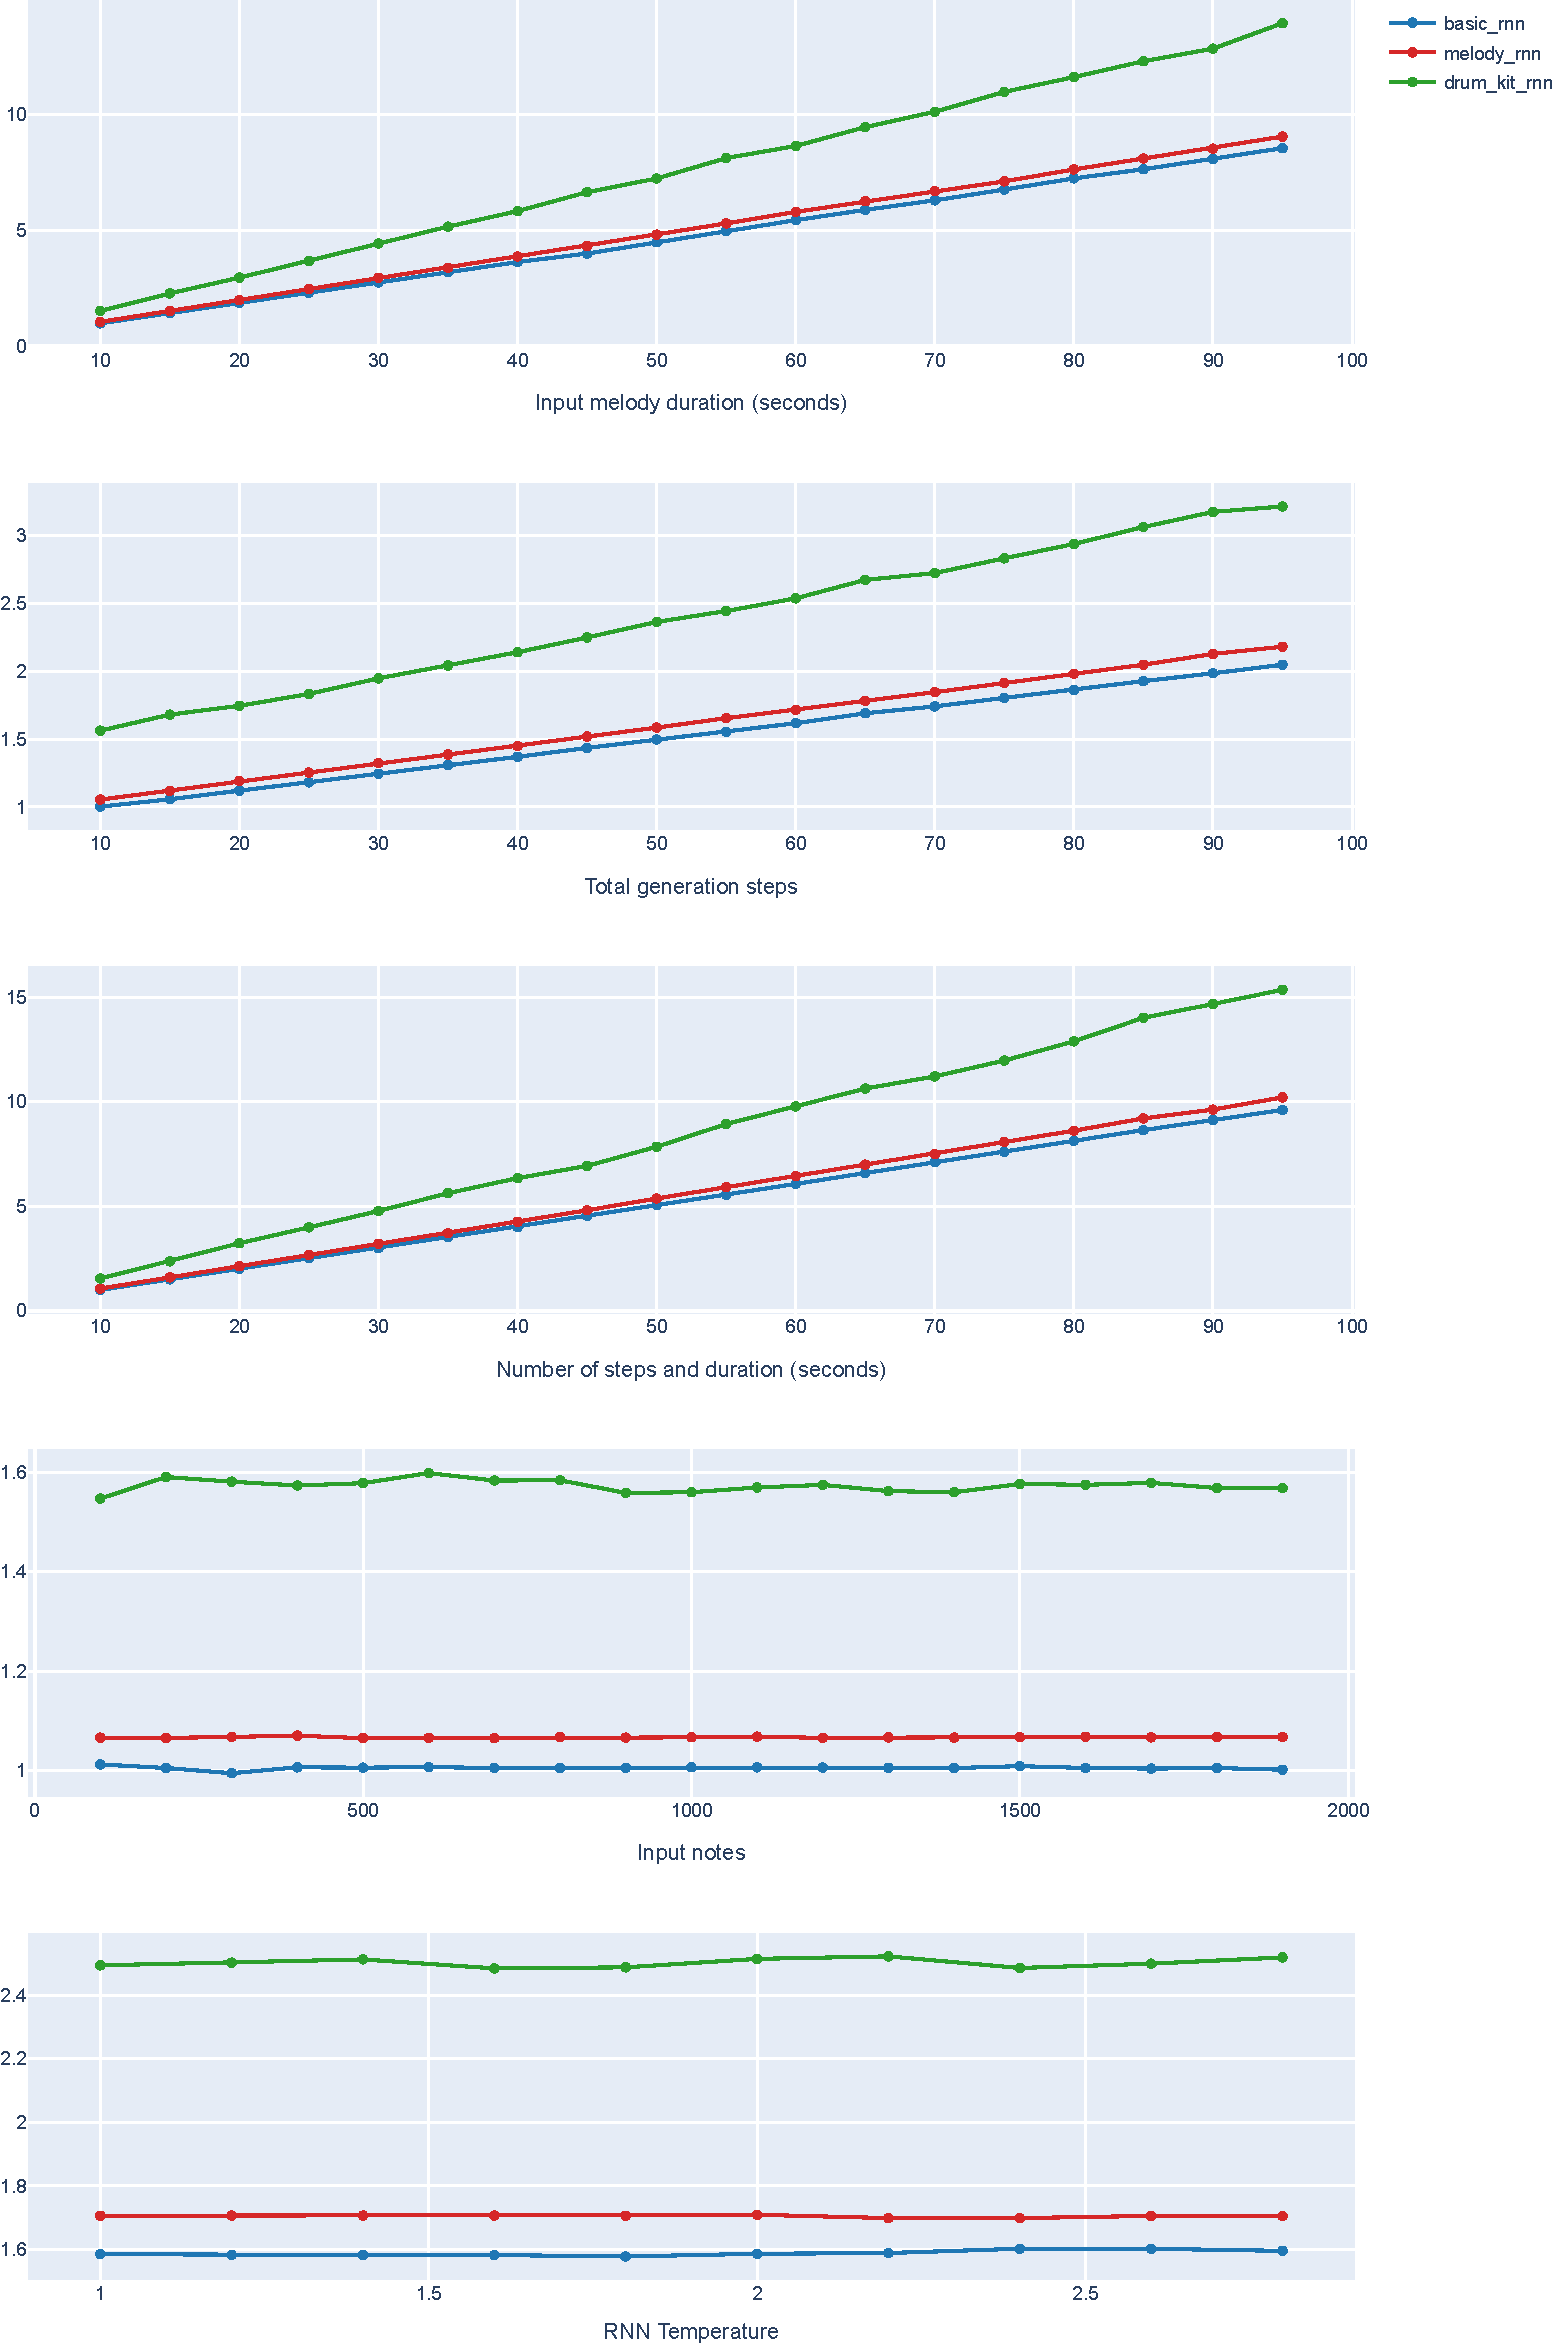
\includegraphics[width=.95\linewidth]{image/perf.pdf} }
  \caption{Magenta Generation Time on the Raspberry Pi 4B}
  \label{fig:magentaperf}
\end{figure}

\paragraph{UI.} It is important to verify that a Raspberry Pi can even run a browser based
DAW with acceptable performance before spending development time creating the web app.
Since we have not developed the DAW at this point, we have tested an existing web based
MIDI editor in the Raspberry Pi.

We used an online MIDI editor called signal (\url{https://signal.vercel.app/}) to get a
subjective feel for the performance. The test was ran in the chromium web browser on
Raspberry Pi OS. The performance was acceptable, with some actions feeling slow.
Dragging around notes had a small but noticeable latency between the mouse cursor's
movement and the notes position. There was also a small but noticeable latency between
double clicking to insert a note and the note showing up on screen. The playhead updated
smoothly when playing the MIDI track, which is the most important aspect, as laggy
playback is awful for the user experience.

It should be noted that this app was not explicitly designed to run on constrained
hardware. Web apps can run great on Raspberry Pis when optimized to do so. Based on our
findings here we are confident that we can develop a browser based app that has
exceptional performance on the Raspberry Pi.

\subsection{MIDI Peripheral}
\label{sec:midi_peripheral}

The Pi needs to function as a MIDI peripheral, i.e. plug the device into a computer and it
functions as a device that sends MIDI commands to the DAW. This connection will happen
through a USB-C to USB-A cable from the Raspberry Pi to the computer. The Raspberry Pi is
typically powered from the USB-C port form a power supply connected to a power outlet, but
in our case the Pi will receive it's power from the host PC over USB-C instead. Once
plugged in, the Pi will act as a normal MIDI peripheral, which sends MIDI events to the
PC, which can be picked up by a fully fledged DAW.

The MIDI communication happens over USB in our case, which means we need to work with the
operating system to send these messages. We are using Linux for our device's operating
system, so USB communication needs to happen through the Linux kernel. This is known as a
USB Gadget in the Linux kernel \autocite{usbGadgetDocumentation}. The Raspberry Pi 4b can
act as a Linux USB Gadget through a USB-C to USB-A connection to the computer, with USB-C
being on the Raspberry Pi and USB-A being on the host computer
\autocite{raspberryPiGadgetSetup}. This will not work out of the box, as the Linux kernel
needs to be made aware that we intend to use the device as a USB gadget. This
configuration happens through files in the \url{/boot/} directory
(see listings \ref{lst:bootconfig} and
\ref{lst:bootcmdline}) \autocite{raspberryPiGadgetSetup}. The Pi will act as a USB
gadget after Linux boot configuration settings are set and it is plugged up to the host
machine.

\begin{minipage}{\linewidth}

  \begin{lstlisting}[language=bash,
  label={lst:bootconfig},
  caption=Lines added to /boot/config.txt \autocite{raspberryPiGadgetSetup, raspberryPiHDMIFix}]
dtoverlay=dwc2
hdmi_force_hotplug=1
hdmi_group=2
hdmi_mode=87
hdmi_cvt=800 480 60 6 0 0 0
hdmi_drive=1
  \end{lstlisting}

  \begin{lstlisting}[language=bash, label={lst:bootcmdline}, caption=DietPi /boot/cmdline.txt modified to allow a USB Gadget \autocite{raspberryPiGadgetSetup}, breaklines=true]
console=ttyS0,115200 console=tty1 root=PARTUUID=8f4dbd00-02 rootfstype=ext4 elevator=deadline fsck.repair=yes rootwait quiet net.ifnames=0 modules-load=dwc2,g_ether
  \end{lstlisting}

  \begin{lstlisting}[label={lst:usb_gadget}, caption=Bash procedure to setup a MIDI Gadget\, modified for our device \autocite{raspberryPiGadgetSetup}, breaklines=true]
cd /sys/kernel/config/usb_gadget/
mkdir -p midi_over_usb
cd midi_over_usb
echo 0x17e8  > idVendor
echo 0xb09c > idProduct
echo 0x0100 > bcdDevice
echo 0x0200 > bcdUSB
mkdir -p strings/0x409
echo "fedcba9876543210" > strings/0x409/serialnumber
echo "MIDI Autofill Group" > strings/0x409/manufacturer
echo "MIDI Autofill Device" > strings/0x409/product
  \end{lstlisting}

\end{minipage}

After the boot configuration options are set, the device will be a USB gadget, but there
is more configuration needed for it to act as a MIDI USB gadget. The Linux kernel already
provides an interface for USB gadgets to act as MIDI devices, through the
\url{usb_f_midi.ko} kernel module \autocite{usbGadgetDocumentation}. We need to set our
Raspberry Pi's USB gadget settings to identify itself as a MIDI peripheral. We have
followed an online guide to setup this MIDI gadget, which involves providing information
to the kernel about our device through the \url{/sys/kernel/config/usb_gadget/} folder
\autocite{raspberryPiGadgetSetup}.

From here we can use the \url{aplaymidi} command to test our MIDI device, which sends a
MIDI file to the host computer \autocite{gadgetTesting}. If the gadget is working
properly, then the MIDI sequences should be visible in any application that listens for
MIDI note events, such as a DAW.

USB Gadgets appear as USB ethernet devices and can be read and written to like any other
networking interface. USB MIDI gadgets similarly communicate through standard networking
interfaces under Linux, meaning that our backend program for sending MIDI events to the
host computer will be sending messages through networking interfaces. However, we will
most likely use a library to abstract away this networking aspect.

USB gadgets work, but we ran into a problem with our setup where our HDMI connection to
the monitor was not working anymore. This connection is critical, as we need to be able to
display our DAW to the built in connection using HDMI, so we had to find a workaround for
this issue. We found out that there are \url{/boot/config.txt} options that can added to
force an HDMI connection, using the \url{hdmi_force_hotplug} option
\autocite{raspberryPiHDMIFix}. This configuration as well as some other HDMI settings can
be seen in listing \ref{lst:bootconfig}.

We have also run into some low voltage warnings when running the Raspberry Pi 4B as a USB
gadget. These warnings are found in system logs and are viewed with \url{journalctl}. The
Raspberry Pi 4b requires 5.1 volts and 3 amps to operate effectively, and will send the
undervolt warning whenever it runs below 4.63 volts \autocite{raspberryPiAmps}. We notice
that we see these warnings early in the boot, but it seems to stabilize later. We have not
run into any issues with these undervolts as of now. The Pi does not encounter anymore
voltage warnings when running a CPU stress test, but it could lead to stability issues
later.  We are still researching  solutions to this problem.


\subsection{Keyboard Design}

\subsubsection{Background}

Any project centered around musicians or their instrument cannot avoid the term ‘feel’. Unlike math or physics where the goal is to arrive at a concrete and unified solution, music is often abstract and expressed through emotions or feelings. There are certainly wrong answers in music, but very few objectively correct answers, and this concept plays a huge role in how musicians choose their instruments.

In a perfect world, the keys of any digital piano (also known as an electric keyboard, keyboard, or synthesizer) would feel, function, and look like an acoustic keyboard: if a player chooses to play a synthesizer, they have most likely played on an acoustic piano. Most keyboard players know that the tactile response of a key in any piano or synthesizer is important because it determines how each note reacts to the player’s touch. For example, lighter keys will respond more quickly to the touch, but will reduce the ease of creating a dynamic range in strike velocity compared to their heavier counterparts. Velocity-sensitive tension spring keys will provide a more uniform tension throughout the keystroke, while weighted keys are balanced on a “balance pin” that separates the user from its striking mechanism, shown in Figure \ref{fig:key_mechanism}, and as a result varies in tension as the key is pressed.

\begin{figure}[h!]
  \centering
  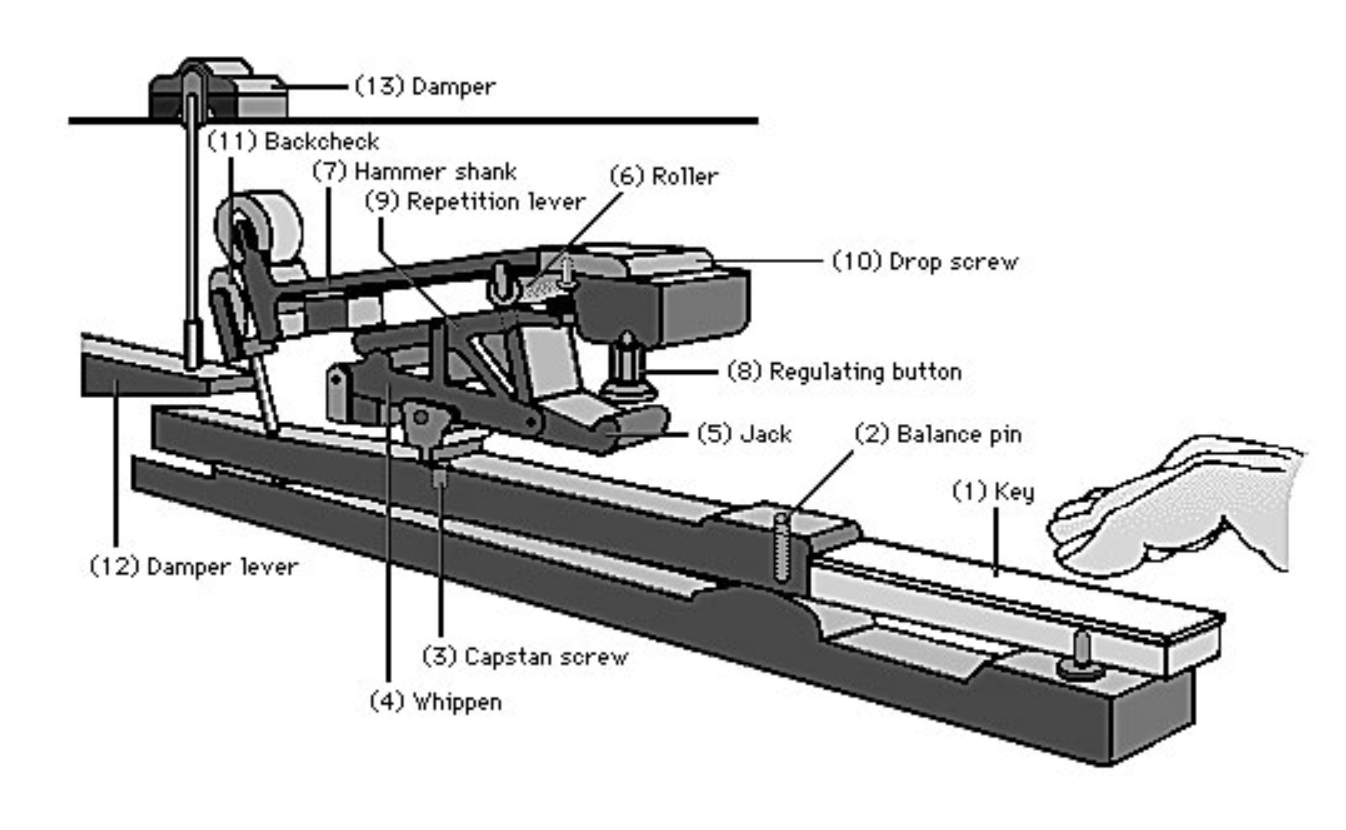
\includegraphics[width=\linewidth]{image/KeyMechanism.png}
  \caption{}
  \label{fig:key_mechanism}
\end{figure}

In addition, each performer and use of the instrument plays a role in determining the desired preference of key feel. EDM or heavily synthesised music designers will care less about key feel because most of the work in writing this type of music, besides determining the melodic structure, will come in post production and adjusting the key inputs from the computer. On the opposite end of the spectrum, classically trained musicians will dramatically care about key feel because most of the work is dedicated to how they express the music through their performance.

On top of the key feel, the amount of keys available to the player has its own important role to the user and their desired end goal as well. To gather a better understanding, a single octave on a piano consists of twelve keys: seven white keys, and five black keys as shown in Figure \ref{fig:octave}. A writer who is focused on beat making and synthesized music can craft most of their music with a single octave and the transposition of that octave. A writer who is classically trained will most likely be adjusted to a standard 7 octave keyboard without the option of transposition. Ultimately, we decided our device should be modeled similarly to a professionally designed MIDI controller that is smaller than five octaves to keep the portability, but larger than one octave to provide a useful range to most players.

\begin{figure}[h!]
  \centering
  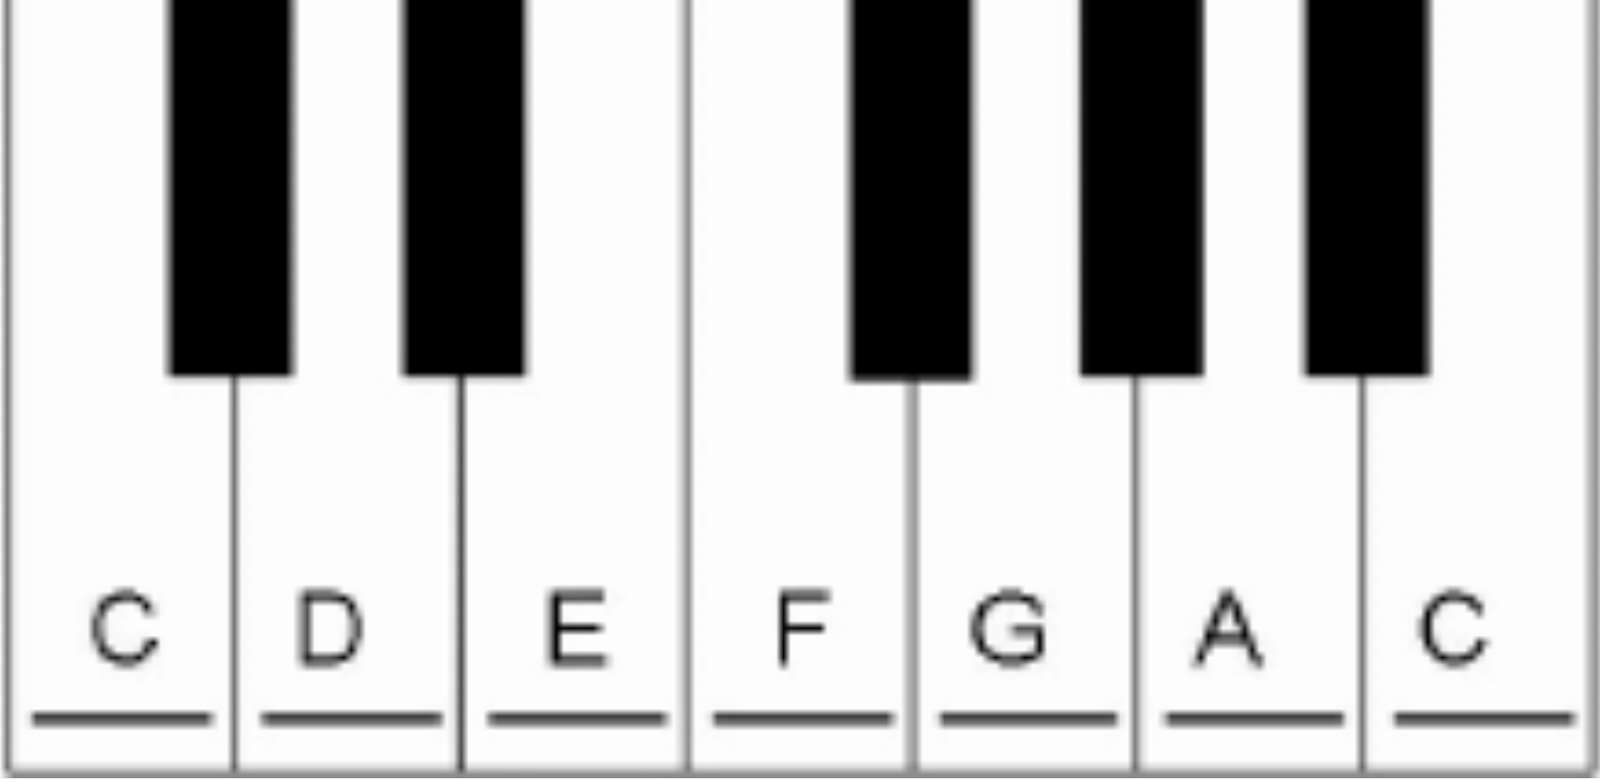
\includegraphics[width=0.5\linewidth]{image/Octave.png}
  \caption{}
  \label{fig:octave}
\end{figure}

\subsubsection{Design}
Our key design was created by referencing two different electric keyboards: the Roland DP-90 and Arturia’s Keylab MkII - 61 key. We chose to measure from these devices because our group has direct access to these and there are no official standardized key sizes. Now, although Figure \ref{fig:octave} does not express the nuances in key design, there are six different key shapes that we have labeled: black, b, t, d, tb, and td, from the letter shapes they are most similar to. tb and tb are a hybrid of the t and b or t and d shape keys. The measurements taken from those devices are shown in Table \ref{Tab:key_specs}.

\begin{table}[h!]
  \centering
  \resizebox{\textwidth}{!}{%
    \begin{tabular}{|l|l|l|l|}
      \hline
      \textbf{Keyboard}       & \textbf{Roland DP-90} & \textbf{Keylab MkII} & \textbf{Our Choice} \\ \hline
      \textbf{Black Key}      &                       &                      &                     \\ \hline
      Base Width (mm)         & 12                    & 12                   & 12                  \\ \hline
      Base Length (mm)        & 95                    & 80                   & 80                  \\ \hline
      Top Width (mm)          & 9                     & 9                    & 9                   \\ \hline
      Top Height (mm)         & 88                    & 72                   & 72                  \\ \hline
      \textbf{Standard White} &                       &                      &                     \\ \hline
      Base Width (mm)         & 22                    & 22                   & 22                  \\ \hline
      Base Length (mm)        & 150                   & 130                  & 130                 \\ \hline
      b cut-in (mm)           & 9                     & 8                    & 8                   \\ \hline
      t cut-in (mm)           & 4.5 / 4.5             & 4 / 4                & 4 / 4               \\ \hline
      d cut-in (mm)           & 9                     & 8                    & 8                   \\ \hline
      tb cut-in (mm)          & 3 / 6                 & 3 / 6                & 3 / 6               \\ \hline
      td cut-in (mm)          & 6 / 3                 & 6 / 3                & 6 / 3               \\ \hline
      Key Separation (mm)     & 1.5                   & 2                    & 2                   \\ \hline
      Trigger Angle (Degrees) & 4.972                 & 5.296                & 5                   \\ \hline
    \end{tabular}}
  \caption{}
  \label{Tab:key_specs}
\end{table}

Our objective is to empower any creative or independent writer, so these devices were happily chosen in particular for their difference in range of use cases. The Roland DP-90 is designed such that it “performs and responds like a grand piano”, while the Keylab MkII is designed as a “definitive MIDI controller keyboard ... a luxurious, expressive tool for your studio” . By taking measurements from two vastly different devices and noticing the minimal variation between their two key sizes, we were able to be confident that our key size choice would suffice. For the project, we chose to go with the cut-in and general measurements of the Keylab MkII because the distance between each key was about 2 mm, compared to the 1.5 mm distance the DP-90 keeps. Since this project will be crafted without professional business assistance, we felt as much leeway to avoid collisions as possible would be beneficial. Additionally, we felt that using the smaller dimensions in key sizes would help reduce the overall form factor of the device and keep it as portable as possible.

We chose to create a thirty-two key keyboard. We landed on this choice as a result of the following factors: first, when this device is in use we do not wish to limit our users to one octave. Our autocomplete AI is modeled from classical music and we understand that the input and output melodies will likely span over a wider range than one octave. We also recognize that this device is more useful in the post-production setting compared to a performance setting and therefore does not need the full seven octave range. Second, to keep the cost low and the form factor small, we wanted to keep the keys below three octaves. We are choosing to build this keyboard as a portable, stand-alone, robust piece of equipment and we believe our device should not cause a struggle to carry around. With the measurements we took, each octave will accompany about 262 mm (10.315 inches) of space in keys alone. This means a thirty-two key keyboard is estimated to need 666 mm (approximately 2.185 ft) of lateral space in keys alone. We knew when multiplexing our signals that using a power of two for our set of inputs would be beneficial. A power-of-two inputs allows us to use the entirety of each multiplexor we implement. As a result, thirty-two keys provides a set of two and a half octaves and will utilize the entirety of each multiplexor without extending the keyboard to sixty-four keys, which is around five octaves. To compare, sixty-four keys would extend to 1290 mm (approximately 4.232 ft) and in our humble opinion, would no longer allow this device to be comfortably portable.

In our application we are looking to distinguish which note is being pressed, the velocity that note was triggered, and which channel the device is communicating through. With the digital functionality of the key in mind, the physical key design only has to worry about how to communicate the velocity of the note. To be able to do this, we are using a two button trigger system for each key. As observed in Figure \ref{fig:key_mechanism}, there are two rods extending from the bottom of the key of different lengths. In the full keyboard model, these rods are lined up with two silicone covered buttons, one of which is triggered at the start of the keystroke and the other is triggered near the conclusion of the keystroke. The difference in trigger time between the two buttons will determine the note velocity which is explained in greater detail from Section [IDK YET].

After basic functionality, our next concern is key feel. With the time allotted for this project and our desire for ease of portability, it is obvious from observing Figure 1 that we will not attempt to replicate the full counter-weighted key design. To keep costs low and durability high, we are also avoiding any semi-weighted keys or the usual expensive key material such as ivory or wood. By utilizing 3D printed plastics, we are able to create custom, robust designs at a cheaper cost than the alternatives.

  [INSERT COST OF MATERIAL AND STRENGTH OF MATERIAL TABLE]

To provide the actuation action for the key itself, we will be using tension springs to hold the key in place as it sits on a lever.
